\subsection{Salvataggio di una Domanda}
	\begin{figure}[h!]
	\begin{center}
		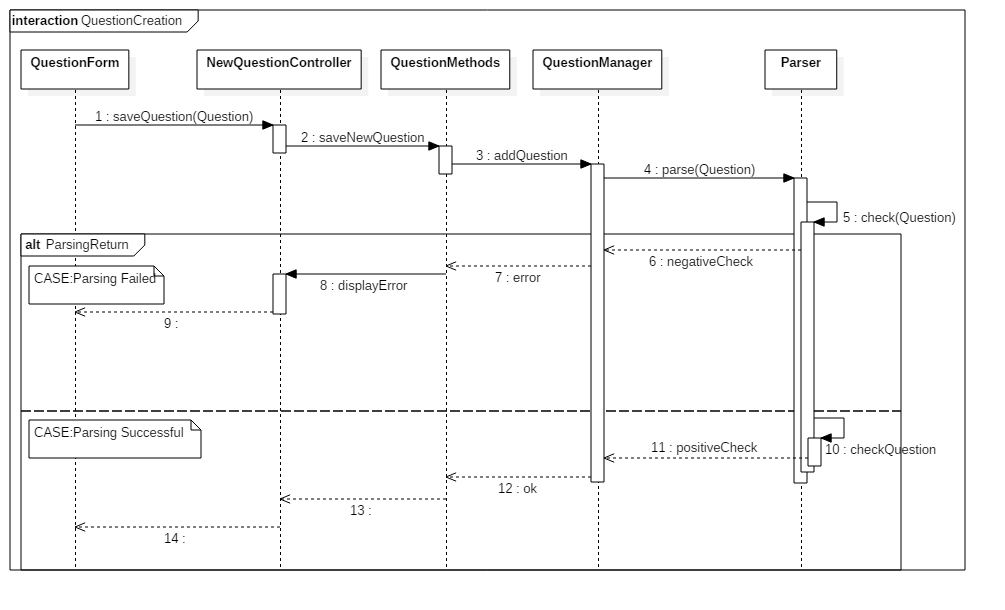
\includegraphics[scale=0.5]{../images/QuestionCreation.png}
		\caption{Diagramma di sequenza del salvataggio di una domanda}
	\end{center}
	\end{figure}
	\begin{itemize}
	\item\textbf{Precondizioni:} l'utente è autenticato nel sistema Quizzipedia e accede all'area del sito dedicata alla gestione (creazione, eliminazione e modifica) dei propri singoli quesiti.\\
	\item\textbf{Postcondizioni:} l'utente ha creato con successo una nuova domanda. La nuova domanda sarà disponibile a tutti gli utenti qualora essi decidano di creare un questionario appartenente alla stessa categoria. L'utente viene reindirizzato alla pagina di gestione questionari.\\
	\item\textbf{Descrizione:} l'utente compila il form per la creazione della nuova domanda (al cui interno ricordiamo è situato un campo adibito alla stesura del codice QML) e sottomette i dati al sistema. L'evento viene notificato alla ViewModel che chiama il Parser situato nel Model passandogli l'input di testo QML. All'interno del Parser viene effettuata la valutazione del codice che può avere due differenti esiti e portare a diversi scenari di conseguenza. In caso il Parser dia un esito negativo, ciò è semplicemente notificato alla ViewModel e di conseguenza alla View che si aggiornerà rendendo noto all'utente il fallimento della procedura di creazione. In caso contrario, ovvero il testo QML inserito dall'utente viene considerato valido, il Model provvede a salvare la nuova domanda nel database (e anche di ciò verrà notificato l'utente con un aggiornamento nella View).\\
	\end{itemize}
	
	\subsection{Visualizzazione e scelta di un Questionario}
	\begin{figure}[h!]
	\begin{center}
		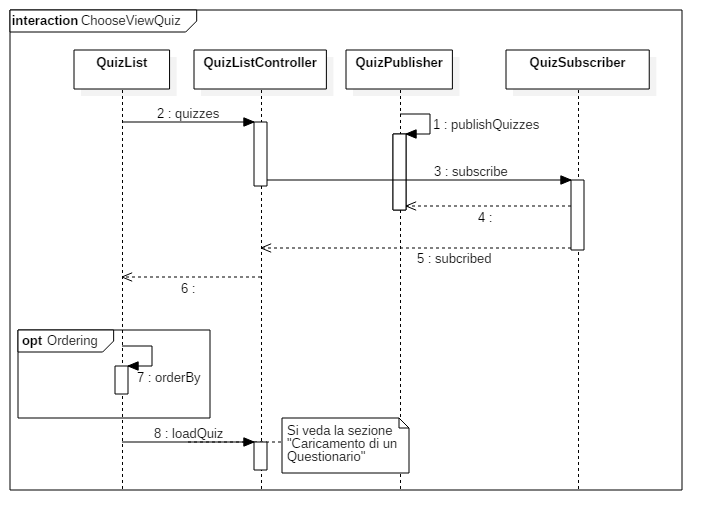
\includegraphics[scale=0.6]{../images/ChooseViewQuiz.png}
		\caption{Diagramma di sequenza sulla visualizzazione e scelta di un questionario}
	\end{center}
	\end{figure}
	\begin{itemize}
	\item\textbf{Precondizioni:} L'utente, intenzionato a svolgere un questionario, accede alla pagina adibita alla selezione dell'argomento.\\
	\item\textbf{Postcondizioni:} L'utente ha scelto un questionario da svolgere e viene reindirizzato alla pagina contenente tale questionario.\\ %è giusta solo questa post o c'è altro?
	\item\textbf{Descrizione:} \textbf{DA CORREGGERE}\textit{La classe CurrentView della View interagisce con la classe InputManager
del Presenter richiedendo un elenco di questionari da visualizzare.} La richiesta viene
inoltrata al Model che procede a recuperare i dati richiesti e a restituirli alla View. Opzionalmente
l’utente ha la possibilità di ordinare i questionari su schermo secondo vari criteri
(alfabetico o cronologico). L’utente ha poi la possibilità di scegliere un questionario e il flusso di eventi si collegherà con quello espresso nel diagramma della sezione "Caricamento
di un Questionario".
	\end{itemize}
	\newpage
	
	\subsection{Caricamento di un Questionario}
	\begin{figure}[h!]
	\begin{center}
		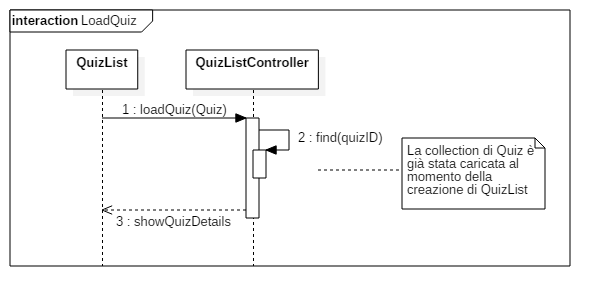
\includegraphics[scale=0.55]{../images/LoadQuiz.png}
		\caption{Diagramma di sequenza sul caricamento di un questionario}
	\end{center}
	\end{figure}
	\begin{itemize}
	\item\textbf{Precondizioni:} L'utente sta entrando in una pagina contenente un questionario che verrà caricato on demand.\\
	\item\textbf{Postcondizioni:} Il questionario è stato correttamente caricato e viene visualizzato a schermo pronto per la risoluzione.\\
	\item\textbf{Descrizione:} L'input iniziale che parte dalla View alla ViewModel contiene l' identificativo del questionario scelto dall'utente. La ViewModel inoltra successivamente questa informazione al Model che si occuperà di estrarre dal database i dati necessari alla costruzione del questionario (effettuata poi dal QuizManager). Una volta assemblato il questionario è pronto per essere somministrato all'utente (il cui diagramma di sequenza è riportato nella sezione "Svolgimento di un Questionario").
	\end{itemize}
	\newpage
	\subsection{Traduzione di una domanda}
	\begin{figure}[h!]
	\begin{center}
		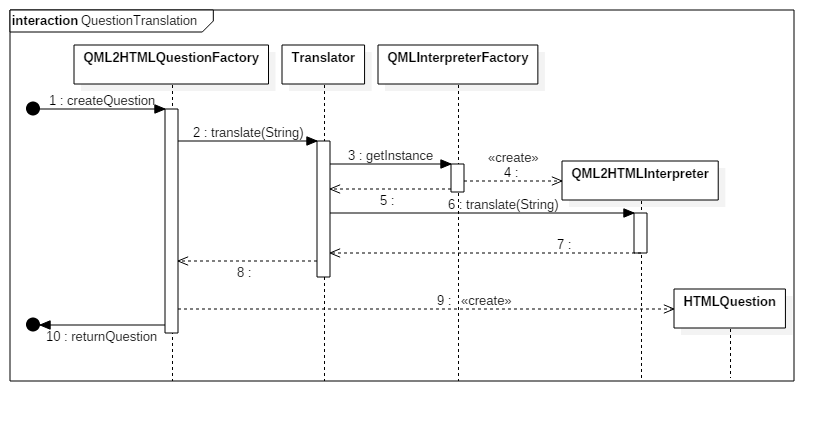
\includegraphics[scale=0.5]{../images/QuestionTranslation.png}
		\caption{Diagramma di sequenza sulla traduzione di una domanda QML}
	\end{center}
	\end{figure}
	\begin{itemize}
	\item\textbf{Precondizioni:} Viene richiesta la visualizzazione su schermo di una domanda.
	\item\textbf{Postcondizioni:} La domanda viene convertita dal precedente formato QML al formato HTML interpretabile dal browser.
	\item\textbf{Descrizione:} alla richiesta di una domanda viene invocata una factory di Question, in questo caso una factory che a partire da testo QML crea domande in HTML. La factory delega la traduzione alla classe Translator; quest'ultima s'interfaccia col package Interpreter, richiedendo l'unica istanza di QMLInterpreterFactory, la quale crea un oggetto QML2HTMLInterpreter. A questo punto Translator può richiedere la traduzione del codice QML all'Interpreter ottenuto, e ritornare il risultato alla QML2HTMLFactory. Infine viene creata la domanda in formato HTML e restituita al richiedente iniziale.
	\end{itemize}
	\newpage
	
	\subsection{Svolgimento di un Questionario}
	\begin{figure}[h!]
	\begin{center}
		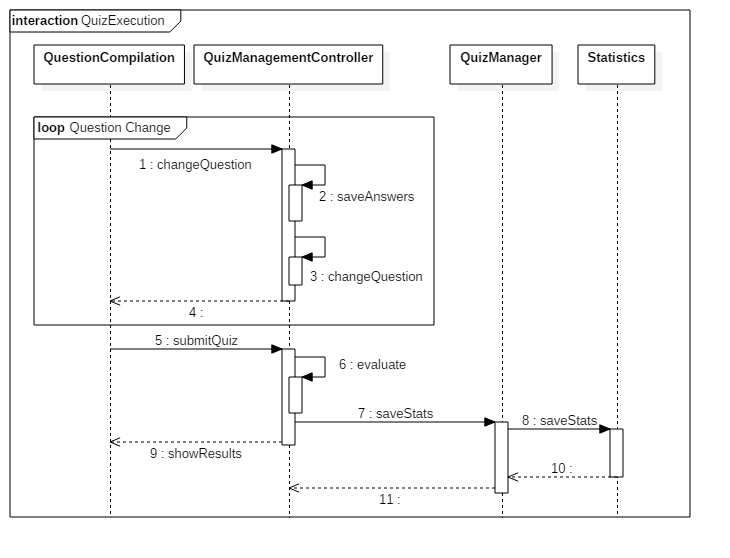
\includegraphics[scale=0.5]{../images/QuizExecution.png}
		\caption{Diagramma di sequenza sullo svolgimento di un questionario}
	\end{center}
	\end{figure}
	\begin{itemize}
	\item\textbf{Precondizioni:} L'utente è intenzionato a svolgere un questionario ed è entrato nella pagina corrispondente a tale questionario. Inizialmente tutte le domande risultano senza risposta. \\
	\item\textbf{Postcondizioni:} L'utente ha svolto il questionario e il sistema, dopo aver compiuto la valutazione, comunica i risultati della prova.\\
	\item\textbf{Descrizione:} Come descritto nel diagramma (evento loop Question Change), l'utente ha la possibilità di scorrere più volte le domande del questionario in modo da risolverle nell'ordine in cui si sente più confortevole. Ogni volta che l'utente richiede la visualizzazione di un'altra domanda il sistema memorizza la risposta fornita dall'utente alla domanda precedente (se questa risposta era effettivamente stata data). Quando un utente ha risposto a tutte le domande può passare alla consegna del questionario, ciò porta al salvataggio delle statistiche della prestazione corrente nella base di dati e al successivo resoconto di valutazione finale che viene esposto all'utente.\\
	\end{itemize}
	\newpage